% crossref 
%\externaldocument{../chapter_2_methods/chapter_methods}
%\externaldocument{../chapter_3_habitats/chapter_habitats}
%\externaldocument{../chapter_4_competition/chapter_competition}

\chapter{Introduction}
\label{Intro}

\section{Social organization across animal species}

The manifold of species, lifestyles, and inhabited ecological nieces that can be found across animal taxa still remains astonishing to scientists and non-scientists alike, even more than a century after Charles Darwin first introduced the concept of evolutionary adaptation. In order to persist under the pressure of natural selection, organisms need to adapt to the different aspects of their environments. With this adaptational process, different forms of social organizations developed across animal species, ranging from animals that stay solitary for most of their life \citep{Cigliano1993, Cornhill2020} to aggregations of several hundreds of individuals, e.g. in large herds of caribous or flocks of birds \citep{Nagy2010, Torney2018}. 

Living in groups can be beneficial, e.g. by means of increasing individual survival chances or reproductive success \citep{Clutton-Brock1999, Sword2005, Bilde2007}. Primarily, this results from the manifold of opportunities to cooperate, e.g. joint territorial and resource defense \citep{Geffen1996, Markham2017}, joint foraging \citep{Hojesjo1998}, shared vigilance and collaborative anti-predator defense \citep{Chivers1995, Clutton-Brock1999, Barber2000, Hass2002, Sword2005}, offspring rearing \citep{DeWoody2000}, etc. On the other hand, groups are more likely to be detected by predators \citep{Cote1995}, their energy expense devoted to foraging is increased \citep{Korstjens2006}, and pathogen and parasite transfer is facilitated \citep{Chapman1995, Cote1995}. Furthermore, individuals in groups also face increased intra-specific competition for limited resources, like food, shelter, or mating partners (e.g. \citealp{Cluttonbrock1979, Janson1985}). The optimal group size for a specific population balances costs and benefits arising from the different aspects of group living. However, these costs and benefits are often distributed unequally, favoring those of higher social status (e.g. \citealp{Janson1985, Wauters1992, Kappeler2008}). Accordingly, rivalries and conflicts between group members are inevitable, wherefore animals developed various mechanisms to economize corresponding social interactions.

\section{Competition and opponent assessment}

Especially in group living species, individuals frequently rival for different limited resources whereby fighting is a key behavior to secure access \citep{Cluttonbrock1979, Chapman1995, Markham2015}. However, competition is costly in terms of energy and time allocated to it as well as an increased risk of injury or death (e.g. \citealp{Briffa2004}). Therefore, individual behavioral decisions during contests are strongly dependent on the associated potential costs and benefits \citep{ArnottElwood2008, ArnottElwood2009}. Often, the best predictor for the outcome of competitions is the contestants' fighting ability, also called resource holding potential (RHP, \citealp{Parker1974}). Usually, larger and stronger individuals win contests since their physical advantages (i.e. higher RHP) directly reflect their increased endurance and potential to inflict damage \citep{Archer1988}. However, additional factors like weaponry, experience, sex, or positional advantages may influence an individual's RHP (reviewed in \citealp{ArnottElwood2008}). 

\begin{figure}[h!]
  \centerline{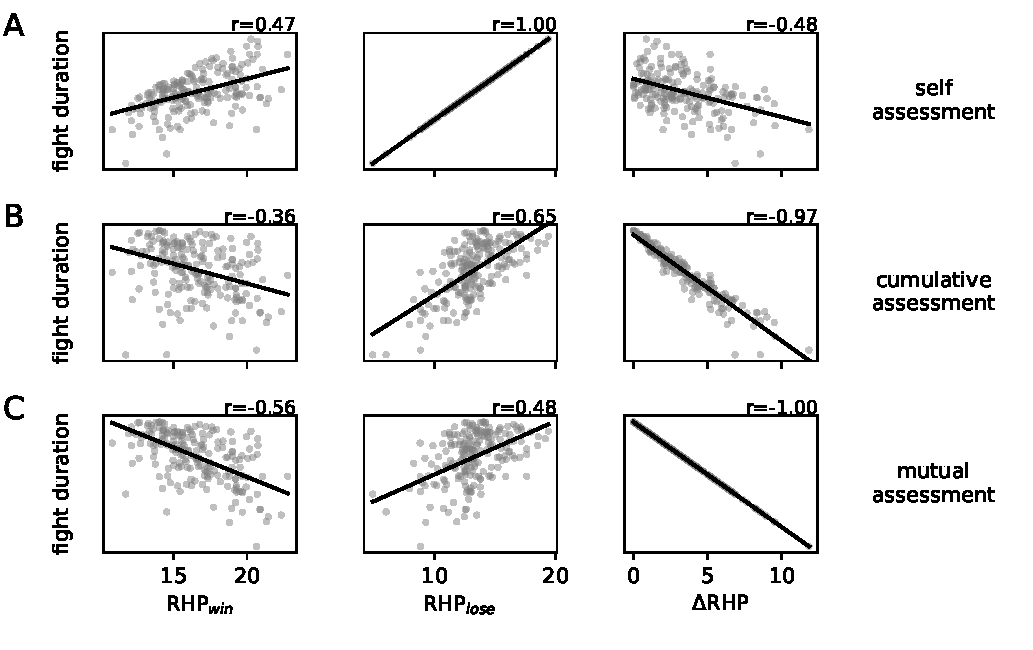
\includegraphics[width=.9\textwidth]{assessment_models_correlations}}
  \caption{\label{assessment_correlations} Dependency of fight duration on the contestants' RHPs and RHP difference ($\Delta$RHP) for different assessment models. Simulations contain competitions between all possible pairings in a population of 1000 individuals with gaussian distributed RHP ($\text{mean}=15$, $\sigma = 3$, only 0.5\,\% shown). P-values of pearson rank correlations were all p$<$0.001. Black lines are linear regressions. For all simulations, costs per second resulting from own actions during competitions ($c_o$) are set to 1\,\textperthousand\, of the mean RHP of the simulated population consistently for all individuals. The amount of damage inflicted by individuals per second ($c_i$) is set to 2\,\% of their own RHP. \figitem{A} Even though the RHP of only the weaker individual (RHP$_{lose}$) is regarded in pure self-assessment (\eqnrefb{self_assessment}), secondary effects, resulting from individuals with higher RHP winning competitions, additionally lead to a positive correlation between fight duration and RHP$_{win}$ and a negative correlation with $\Delta$RHP respectively. Fight duration increases with RHP$_{lose}$ as expected. \figitem{B, C} In contrast, RHPs of both contestants are regarded in cumulative assessment (panel~\panel{B}, \eqnrefb{cum_assessment}) and mutual assessment (panel~\panel{C}, \eqnrefb{mutual_assessment}). In both cases, fight duration increases with RHP$_{lose}$ and decreases with RHP$_{win}$ and $\Delta$RHP, complicating their differentiation. For simulated competitions assuming mutual assessment, fight duration is assumed to linearly increase with increasing $\Delta$RHP, i.e. in \eqnrefb{mutual_assessment}, the exponent $\alpha$ describing the link between $\Delta$RHP and fight duration equals 1.}
\end{figure}

\begin{figure}[t]
  \begin{minipage}[t]{0.66\textwidth}
    \mbox{}\\
    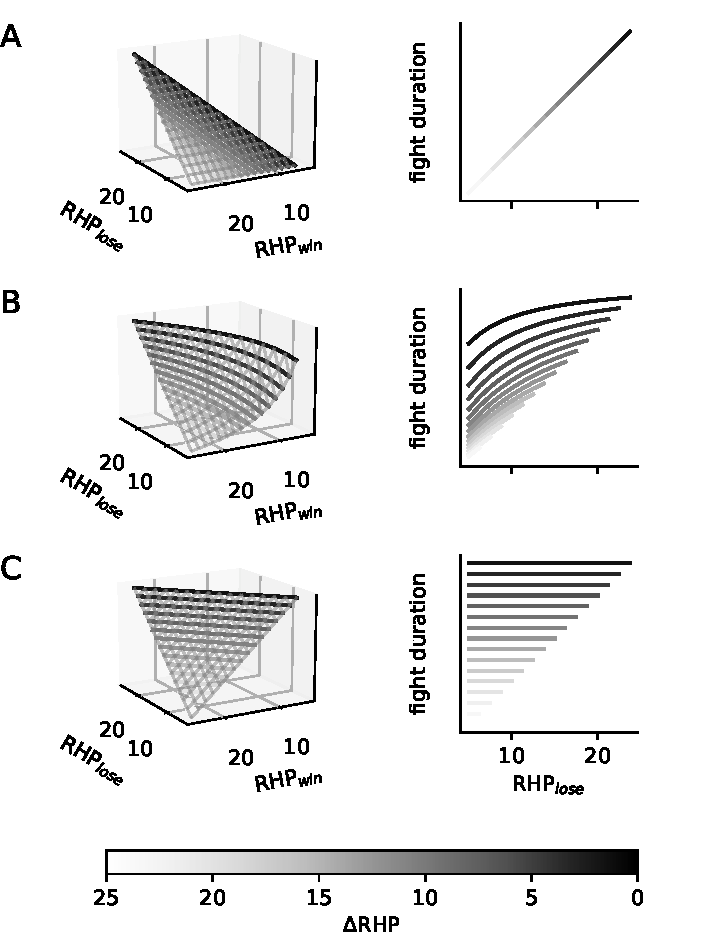
\includegraphics[width=1\textwidth]{assessment_model_simulation}
  \end{minipage}\hfill
  \begin{minipage}[t]{0.3\textwidth}
    \caption{\label{assessment_sim} At fixed RHP differences ($\Delta$RHP), the relation between fight duration and a contestant's RHP varies across assessment models. Panels on the left show how both RHP$_{win}$ and RHP$_{lose}$ influence contest duration ($\Delta t$, z-axis) across the different assessment models, i.e. the basis for simulations shown in \figref{assessment_correlations}. Right panels display the correlation of contest duration and RHP$_{lose}$ for fixed $\Delta$RHP values (grey scale). \figitem{A} In pure self-assessment, the correlation of fight duration and RHP is unaffected by $\Delta$RHP. \figitem{B} In cumulative assessment, fight duration increases with RHP for defined $\Delta$RHPs. \figitem{C} In mutual assessment, fight duration remains unaffected by the contestants' RHP at fixed $\Delta$RHP.}
  \end{minipage}
\end{figure}

The course of competition and associated behaviors have been shown to be either based on the assessment of solely a competitor's own RHP or by integrating both the own and opponent's RHP \citep{Enquist1990, Taylor2001, Huyghe2005}. In the first case (self-assessment), costs resulting from competition are accumulated until an endurance threshold, set by an individual's RHP, is reached and the respective individual retreats \citep{ArnottElwood2009}. In self-assessment models, competition costs arise either exclusively from own behaviors (pure self-assessment, \citealp{Taylor2003}) or are additionally supplemented by costs inflicted by opponents (cumulative assessment, \citealp{Payne1998}). In both cases, no direct information about an opponent and its RHP is gathered. Alternatively, in mutual assessment the contestants assess each other's RHP, compare it to their own, and adjust their behavior according to the difference \citep{EnquistLeimar1987}. The huge benefit of this strategy is its economic efficiency. Individuals can recognize their inferiority and retreat long before their endurance threshold is reached, thereby saving metabolic costs for both competitors. However, which assessment model is utilized in competitions of a given species is dependent on the associated costs and benefits. Sometimes the costs of continuous assessment are too high, favoring pure self- or cumulative assessment. In other cases, costs of escalating physical fights are too high to be justified by the benefits of a certain resource, thus favoring mutual assessment \citep{ArnottElwood2009}. In order to experimentally identify which form of assessment is utilized during competitions in a given species, it is necessary to rely on the evaluation of associated behavioral manifestations, e.g. how fight duration depends on the contestants' physical attributes or RHP. However, the intuitive interpretation of corresponding data is extremely error-prone. For example, mutual assessment has previously often been assumed solely because of a negative correlation between the contestants' RHP difference ($\Delta \text{RHP} = \text{RHP}_{win} - \text{RHP}_{lose}$) and fight duration (reviewed in \citealp{ArnottElwood2009}). However, secondary effects resulting from individuals with higher RHP usually winning competitions consistently lead to negative correlations between RHP difference ($\Delta$RHP) and fight duration across all assessment models (\figref{assessment_correlations}, right).  

\subsection{Simulating assessment models}

Divergences between the different assessment models can be determined in simulated competitions between contestants of different RHP. The basic assumption for these simulations is that during competitions, costs arising from own actions per time (c$_o$) remain constant and independent from an individual's own RHP, whereas costs inflicted to opponents per time (c$_i$)
\begin{equation}
\label{inflicted_costs}
c_i = \beta \cdot \text{RHP}
\end{equation}
increase with increasing RHP by a factor $\beta$. Accordingly, we set competition costs per second arising from own actions to 1\,\textperthousand\, of the mean RHP of a simulated population of 1000 individuals ($\text{mean RHP} = 15$) consistently for all individuals and costs inflicted per second to 2\,\% of a competitor's own RHP respectively. 

For pure self-assessment, the duration of competitions can be simulated as 
\begin{equation}
\label{self_assessment}
\Delta t = \frac{RHP_{lose}}{c_o}.
\end{equation}
Accordingly, this model is the only one solely regarding information about one competitor, i.e. the weaker individual. On the contrary, the simulated duration of competitions assuming cumulative assessment
 \begin{equation}
\label{cum_assessment}
\Delta t = \frac{RHP_{lose}}{(c_o + c_i)}
\end{equation}
or mutual assessment
\begin{equation}
\label{mutual_assessment}
\Delta t = D - (RHP_{win} - RHP_{lose})^{\alpha}
\end{equation}
with D corresponding to the maximum observed fighting duration and $\alpha$ to an exponent describing the link between RHP difference and fight duration, both incorporate information about both contestants' RHPs, either directly (mutual assessment: RHP$_{lose}$, RHP$_{win}$) or indirectly (cumulative assessment: RHP$_{lose}$, c$_i$). 

According to our simulations, pure self-assessment can be distinguished from the other models by positive correlations of contest duration with both contestants' RHP (strong for RHP$_{lose}$, weaker for RHP$_{win}$) and a negative correlation of contest duration with the contestants' RHP difference ($\Delta$RHP, \figrefb{assessment_correlations} upper panels). However, differentiating cumulative from mutual assessment requires further investigation since correlations between contest duration and absolute or relative RHPs are rather similar (\figref{assessment_correlations} central and lower panels). Nevertheless, in mutual assessment competitions between contestants of a given $\Delta$RHP last equally long independent from the contestants' individual RHPs (\subfigref{assessment_sim}{C}), whereas the basic assumption of cumulative assessment leads to competitions between contestants of a given $\Delta$RHP to last longer for contestants with higher absolute RHP (\subfigref{assessment_sim}{B}). Another criterion to distinguish cumulative from mutual assessment is the procedure of competition itself. While contests under the assumption of mutual assessment occur in discrete phases (repetitive assessment of contestants to acquire a better estimate of an opponent's RHP relative to their own, \citealp{EnquistLeimar1987, Enquist1990}), contests including cumulative assessment usually occur and escalate in a single phase \citep{Payne1998}. 

\section{Dominance and social hierarchies}

In natural populations, individuals are likely to encounter and rival with the same individuals repeatedly. Instead of accumulating the high costs arising from repetitive fighting (e.g. \citealp{Briffa2004}), many species rather use these competitions to establish dominance hierarchies, where access to resources, e.g. food and mating partners, is determined by social rank. By means of specific cues and/or actively generated signals, group members can assess each other's social status in a cost-efficient way (e.g. \citealp{Cluttonbrock1979, Fernald2014, Cornhill2020}). This accordingly reduces the necessity of fighting over resources and is therefore beneficial for all individuals involved \citep{Cluttonbrock1979, Janson1985, Creel1996}. Nevertheless, access to resources is asymmetric in dominance hierarchies, favoring those of higher social rank \citep{Janson1985, Wauters1992, Sapolsky2005, Taves2009}. Associated benefits for dominants include increased reproductive success, higher net food intake, decreased predation risk, and much more (e.g. capuchin monkeys: \citealp{Janson1985, Jason1990}, wallabies: \citealp{Blumstein2001}, hyenas: \citealp{Engh2002}, mandrills: \citealp{Charpentier2005}, lemurs: \citealp{Kappeler2008}). Subordinates, on the other hand, often have to accept compromises and adjust their behavior according to their social rank, e.g. forage lower quality patches at the rear of the group at the expense of increased predation risk (e.g. \citealp{Jason1990}). However, subordinates still profit from the general benefits of living in groups and also receive less aggression compared to corresponding individuals in populations of species not forming dominance hierarchies at all \citep{Sapolsky2005}. Still, this asymmetric access to resources can lead to situations where for subordinates, the individual costs of living in a group outweigh the benefits. For the respective animals, emigration into another group can be beneficial since it can potentially lead to social advancements, e.g. an increase in relative social rank \citep{Janson1985, Chapman1995, Markham2017}. Minnows, for example, indeed tend to join groups of individuals with lower competitive abilities \citep{Metcalfe1995}.

The specific characteristics and manifestations of dominance hierarchies vary greatly across the animal kingdom, depending on a species' way of life and ecological factors \citep{Janson1985, Cigliano1993, Sapolsky2005}. While in group-living species complex social structures can emerge, e.g. the development of a leader-follower dynamic \citep{Strandburg2018}, dominance in solitary species is rather associated with resource based benefits, e.g. the occupation of higher quality territories and increased reproductive success (e.g. \citealp{Cigliano1993}). Differences in the abundance and dispersion of food and other resources can further lead to variation regarding the skewness in access to resources across social ranks. In bottom-up egalitarian hierarchies, resources are more equally distributed \citep{Sapolsky2005}, whereas in top-down despotic hierarchies, access to resources is strongly skewed in favor for dominant individuals \citep{Kappeler2008}. Despotic hierarchies can be reinforced by harsh environmental conditions, e.g. very limited resources. As a consequence of this increased environmental compulsion, dominants show increased levels of agonistic actions (displays and attacks) in order to preserve their social status and associated benefits. However, this leads to increased levels of stress for all individuals compared to more egalitarian dominance hierarchies and represents an additional cost of group living for the affected animals \citep{Janson1985, Creel1996, Cavigelli1999, Sapolsky2005, Kappeler2008}.


\section{Animal communication}
Animals constantly gather information from their sensory periphery and adapt their behavior accordingly. In addition to the perception and interpretation of passive environmental cues, animals can gather and share information by means of actively emitted communication signals (e.g. \citealp{Demartsev2018, Cornhill2020, Ritschard2010}). Such signals can convey important social and environmental information which otherwise would not be available for receiving individuals. Accordingly, they can reduce the uncertainty inherent in different situations, especially social interactions, and thereby facilitate behavioral decision-making, which is usually beneficial for both sender and receiver of a signal. Neither would a sender emit a signal, nor a receiver respond to it if it was not beneficial for them \citep{Seyfarth2017}. Thus, communication is shaped by natural selection and is adaptive for both sender and receiver.

Animals show an enormous diversity in whether, where, when, and how they communicate. This huge diversity results from signal properties being adapted to their specific signaling purpose as well as the sensory and communicative characteristics of the respective animal species utilizing them (e.g. \citealp{Fernald2014}). For example, the utilization of urine marks as chemical signals are most suitable to signal status and territorial occupation in rather solitary living species with huge territories because of their longevity  \citep{Cornhill2020}, whereas distinct short living acoustic or visual signals are most suitable in contexts aiming for immediate responses by receivers, e.g. group cohesion calls \citep{Demartsev2018}, predator alarm calls \citep{Schibler2007}, or mating signals \citep{Ligon2018}. \citet{Bandbury2011} classified communication signals according to their behavioral context into four categories: aggressive signals (e.g. threats, territorial or dominance signals, \citealp{Cluttonbrock1979, Kappeler2008, Fernald2014, Bolt2019, Kareklas2019, Cornhill2020}), mating signals \citep{Ritschard2010, Henninger2018, Ligon2018}, social integration signals (e.g. group cohesion or reconciliation, \citealp{Cheney1995, Schamberg2016, Demartsev2018}) and environmental signals (e.g. signaling presence and/or location of predators or food, \citealp{Seyfarth1980, Seeley1997, Schibler2007}). 

The specific information which animals can gather or share using communication signals depends to some extent on specific signal properties \citep{Seyfarth2003}. In order to be evolutionary stable, signals need to yield a predictable relation to a specific individual or a specific social or environmental situation (informative value). For example, alarm calls indicate the presence of a specific predator \citep{Seyfarth1980}, or the frequency of red deer roars or toad croaks reliably indicates body size and competitive abilities \citep{Davies1978, Reby2005}. The direct informative value of a signal is further enhanced when only a narrow band of stimuli elicit the corresponding signal (referential specificity) and/or the signal is well distinguishable from other signals (signal specificity, \citealp{Seyfarth2003}). However, the development and emission of a multitude of distinct signals is costly. Therefore, signals are only further refined when the corresponding evolutionary benefits outweight these costs (e.g. refinement of predator alarm calls, \citealp{Schibler2007}). Accordingly, most signals usually do not fulfill all three criteria for highly specific and informative signals (i.e. high informative value, referential specificity, signal specificity) and are rather vague in at least one of the stated dimensions. Detailed information can, nevertheless, be gained from these rather vague signals by incorporating contextual information. Communication does not occur in a social or environmental vacuum, but rather in stereotypical situations, where the range of possible signal interpretations is limited. For example, wild baboons \textit{Papio cynocephalus ursinus} use the same "grunts" to coordinate group movement, signal their intention to handle infants of other mothers, as well as to reconcile after aggressive encounters \citep{Cheney1995, Rendall1999}. Similarly, the electric fish \Lepto{} uses the same electocommunication signal, so called "chirps", both during aggressive same-sex encounters and during courtship \citep{Henninger2018}. Thus, by incorporating contextual cues, animals can obtain precise information even from rather vague signals \citep{Seyfarth2017}, reducing the necessity of further costly signal refinement \citep{Schibler2007}.

In captivity or isolation, the communicative behavior of animals often deviates from their natural behavior, presumably because of missing naturalistic contextual cues. In isolation, baboon grunts are very general, non-specific signals \citep{Cheney1995, Rendall1999} and also the electrocommunication behavior of \lepto{} shows great divergences between confined laboratory experiments and observations in naturalistic experiments or in the wild \citep{Henninger2018}, to remain with those two examples. Accordingly, to understand animal behavior and especially the functionality of communication signals, the incorporation of context into behavioral evaluation is indispensable \citep{Seyfarth2017}, which is especially important and needs to be regarded in order to design valid laboratory experiments.

\section{Methodological approaches for behavioral studies}

Determining the causality of animal behavior in experimental or observational studies is often challenging since animals are sensitive to a broad range of stimuli. Animals adapt their behavior according to their current social and/or environmental surrounding (e.g. \citealp{Chapman1995, Sapolsky2005, Markham2015}) as well as to their own internal state and needs (e.g. \citealp{Boon2007}). Therefore, experimental conditions of laboratory experiments that often comprise reduced and unnatural environments can influence animals and lead to divergences between behaviors observed in the laboratory and those observed in the wild (e.g. \citealp{Cheney1995, Rendall1999, Henninger2018}). On the other hand, identifying, monitoring and regarding all factors affecting animal behaviors observed under naturalistic conditions is simply impossible.

\begin{figure}[h!]
  \centerline{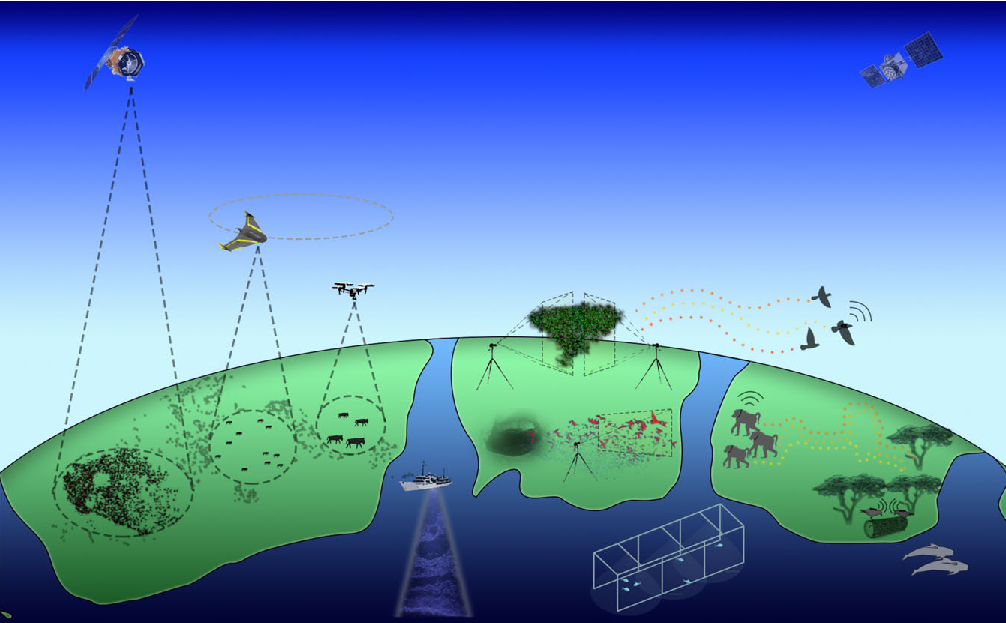
\includegraphics[width=.8\textwidth]{methods_behavioral_studies}}
  \caption{\label{methods_hebavioral_studies} Different methodological approaches emerged from the rapid technological advances of the last decades. Recording devices range from satellites, over unmanned aerial vehicles like drones, to stationary single or synchronized cameras and animal mounted bio-loggers. This huge variety of recording devices enables data acquisition to be adapted to the requirement of a scientific study, i.e. a specific model species, its behavior, the environmental conditions it lives in, and the scientific question that shall be tackled. Taken from \citet{Hughey2018}.}
\end{figure}

However, recent technological advantages in remote recording techniques, tags, and data loggers (\figref{methods_hebavioral_studies}), as well as in associated data processing techniques enable high-throughput studies not only for behavioral sciences but also for ecology and neuroscience \citep{Anderson2014, Dell2014, Hughey2018, Mathis2018}. A benefit of these approaches is that recordings contain rather unspecific data from which all sorts of information can be retrieved after the recordings have been made, including behavioral events or environmental information \citep{Gomez2014}. This allows for post-hoc discoveries of behavioral causalities and the development of associated hypotheses, which has already been demonstrated in research on group coordination in baboons \citep{Strandburg2015} and meerkats \citep{StrandburgPeshkin2019}, as well as reproductive behavior in field crickets \citep{Rodriguez2010}. 

Based on the requirements of a scientific project, i.e. model species, environmental conditions, and scientific question, the most suitable recording technique can be selected from a huge variety of available recording devices \citep{Hughey2018}. Respective methodological approaches can be subdivided into two main categories: Either animals themselves are equipped with bio-loggers or external recording devices are utilized to record their behavior.

\paragraph{Bio-loggers} 

Bio-loggers are small devices that, equipped with a variety of different on-board sensors, get affixed to animals themselves and record different aspects of their behavior or physiological condition \citep{Menzel2005, Baktoft2015, Strandburg2015}. Accordingly, they are most suitable to study highly mobile animals or those who live in remote, hard to access areas. Using this method, many interesting insights into different aspects of natural animal behavior have been gained already, including collective movement \citep{Nagy2010, Strandburg2015}, leadership \citep{Strandburg2018}, or foraging ecology of deep-diving animals (elephant seals: \citealp{Robinson2012}). 

Still, technical limitations of bio-loggers can lead to some issues that can potentially influence scientific validity. Experimenters frequently need to interact with animals (e.g. to mount, recharge, or read-out loggers) and animals are required to carry recording devices. This alone already can result in changes of behaviors, reproduction, or survival, and thus bias observations \citep{Saraux2011}. In order to reduce these biasing factors, different trade-offs regarding sample rate, duty cycling, and battery life are required \citep{Hughey2018}, e.g. the deployment of smaller loggers that have less effects on an animal's natural behavior at the cost of decreased battery capacity or devices recording discontinuously for predetermined time periods in order to reduce energy consumption and therefore the frequency of required interactions with animals (e.g. \citealp{StrandburgPeshkin2017}). Furthermore, not all individuals of a study population can usually be equipped with recording devices (e.g. \citealp{StrandburgPeshkin2019}) and those loggers deployed are limited in their recording range to the direct surrounding of the respective animal. Accordingly, bio-loggers can potentially miss out on recording relevant stimuli that elicit recorded behaviors when (i) stimuli take place off recording cycle or (ii) out of detection range of deployed bio-loggers, with the latter also including (iii) untagged animals. 

These unavoidable trade-offs have the potential to impede the validity of respective studies, which might even remains unnoticed. For example, when conducting behavioral studies in natural populations, possible changes in the composition of the study population have to be regarded, e.g. caused by individuals leaving or joining the group \citep{Janson1985, Engh2002}. Such changes can have tremendous effects on group or individual behaviors \citep{Metcalfe1995, Sapolsky2005}. However, with incompletely tagged groups, the detection of such events can be difficult or impossible and the evaluation of recorded behaviors elicited by such undetected events can lead to the suggestion of false causalities.

\paragraph{Remote-sensing} 
An alternative approach is to refrain from animal mounted bio-loggers and instead detect and track whole populations of animals and their behaviors in external recordings \citep{Hughey2018}. Corresponding devices can be anything capable of recording different aspects of an animal's morphology or behavior, including satellites, unmanned aerial vehicles equipped with on-board sensors (e.g. drones with video cameras), stationary synchronized or single video-cameras, directed microphones, or even arrays of electrodes submerged in the water \citep{Theriault2014, Henninger2018, Hughey2018}. Even though these techniques are sometimes disadvantageous in natural, cluttered environments \citep{Dell2014} the huge versatility of recording devices allows for their utilization in the context of various different studies. Individual flight paths of bats and birds have been reconstructed from video recordings of stationary cameras \citep{Theriault2014}, herds of caribous have been filmed using unmanned aerial vehicles like drones in order to study collective movement and information transfer in groups \citep{Torney2018}, and electric signals of electric fish have been recorded using electrode grids to gain insights into their natural communication and movement behaviors \citep{Henninger2018, Henninger2020}. However, the evaluation of such recordings is way more challenging compared to bio-loggers. Recorded animal signals (e.g. aspects of appearance or emitted signals) need to be detected, classified, and tracked in order to obtain viable behavioral traces. This usually requires custom analysis tools that are adapted to a specific scientific question (e.g. individual or species identification, behavioral classification, etc.).

\paragraph{Laboratory studies} 
Indeed, observations and experiments in an animal's natural environment are indispensable in order to fully understand their behaviors, since only there the entirety of stimuli and circumstances potentially affecting them is available. Nevertheless, laboratory studies are of central interest, too, since they allow for detailed and continuous observations of behaviors in response to well controlled stimuli (e.g. \citealp{Chivers1995, Barber2000, Hupe2008}). Accordingly, causalities between behaviors and different stimuli can easier be identified and described more accurately. However, as mentioned above, behaviors observed in the laboratory often severely deviate from natural behaviors, because of artificial experimental conditions \citep{Henninger2018}. 

Laboratory experiments with long and continuous observation times in semi-naturalistic environments can combine the advantages of well controlled laboratory experiments and field observations. Diverse aspects of an animal's behavior can be observed in depth, while naturalistic environmental conditions ensure behaviors to be much closer to those observed in the wild. Unfortunately, studies of these kind are still rare, though, since handling and analysis of the resulting large and high dimensional data-sets is demanding and challenging \citep{Gomez2014}.

Yet, electric fish are most suitable for such elaborate studies. These fish emit electric signals that can be recorded by means of electrode arrays submerged in the water and used for tracking individual behaviors, including communication \citep{Smith2013} and movement \citep{Madhav2018, Henninger2020}. Since this method is non-invasive, recorded behaviors can be assumed to be most natural, especially when fish are kept under naturalistic conditions. Furthermore, long-term behavioral observations are feasible in these fish since recording duration is only limited by data storage capacities.

\section{Electric fish}

\begin{figure}[h!]
  \centerline{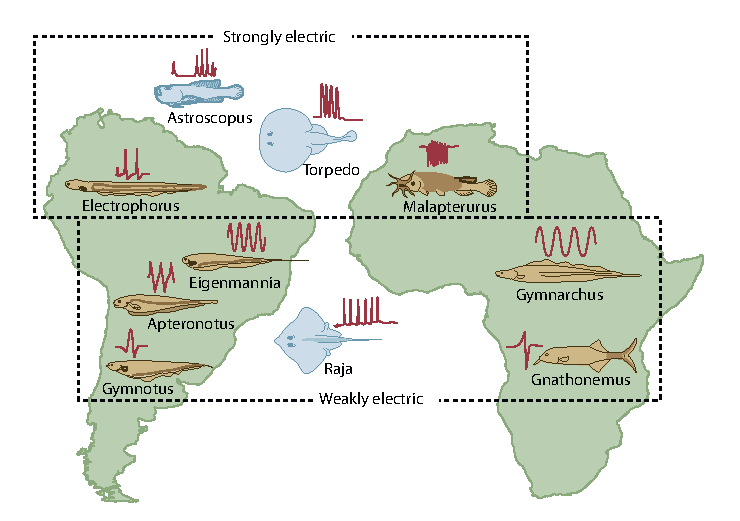
\includegraphics[width=.8\textwidth]{distribution_efish}}
  \caption{\label{efish_dist} Global distribution of electric fish species. Different species can be found in marine (blue) as well as in freshwater (yellow) environments. Species specific EOD wave-forms are above the respective sketches (red). While strongly electric fish are capable to stun their prey, weakly electric fish utilize their electric fields for electrolocation and communication. Taken from \citet{Nelson2011} after \citet{Moller1995}.}
\end{figure}

Two groups of electric fishes (African Mormyriformes and South American Gymnotiformes, \figrefb{efish_dist}) have independently developed electrical organs, producing species specific electric organ discharges (EODs, \citealp{Hopkins1978, Turner2007}), used for electrolocation \citep{Nelson1999, Fotowat2013} and communication \citep{Smith2013}. In particular, Gymnotiform wave-type fish continuously generate EODs with individual-specific frequencies that remain, in constant environments, remarkably stable over many hours and days (\citealp{Bullock1970, Moortgat1998}, \figsrefb{efish_dist}, \subfref{field_simulation}{B}). That is, these fish all “glow” in individual “colors”. By simply recording their electric fields with an array of electrodes submerged in the water -- as has been suggested by \citet{Hagedorn1985} -- these fish can be tracked without the need to tag them or to mount loggers \citep{Jun2013, Matias2015, Madhav2018, Henninger2018, Henninger2020}. Furthermore, electrocommunication signals (see below) are recorded in one and the same channel which is also used for tracking \citep{Henninger2018}. This makes electric fish an advantageous and highly accessible model organism for large-scale and detailed behavioral observations.

Species diverse Gymnotiform fishes (more than 250 species, \citealp{Albert2005, Ferraris2017}) make up to 70\,\% of the biomass of large rivers in South America \citep{Marrero1991, Cox2004, Crampton2011}. However, despite their importance in tropical freshwater ecosystems \citep{Cox2004, Crampton2011} and their extensively studied electrosensory system \citep{Benda2005, Bullock2006, Grewe2017, Sinz2020}, little is known about their ecology, ethology and life history, because field research on these fascinating fishes was, until recently, severely limited by their nocturnal and secretive lifestyles. During the day, electric fish hide at resting sites under submerged logs (Gymnotus, \citealp{Westby1970}), between roots (Eigenmannia, \citealp{Hopkins1974}), within leaf litter (Brachyhypopomus, \citealp{Hagedorn1988}), and even buried in sand (Gymnorhamphichthys, \citealp{Lissmann1965}). During the night, however, these fish become more active: Some species increase their EOD frequency (EODf, \citealp{Lissmann1965, Stoddard2007}), communication signals are produced more frequently \citep{Zupanc2001, Henninger2018}, higher movement activities can be observed \citep{Henninger2020}, and courtship takes place \citep{Hagedorn1985, Henninger2018}. Altogether, a plethora of behaviors and social interactions can be observed in these fascinating animals during the night.

\subsection{\Lepto{} and its social behavior}

\begin{figure}[h!]
	\centerline{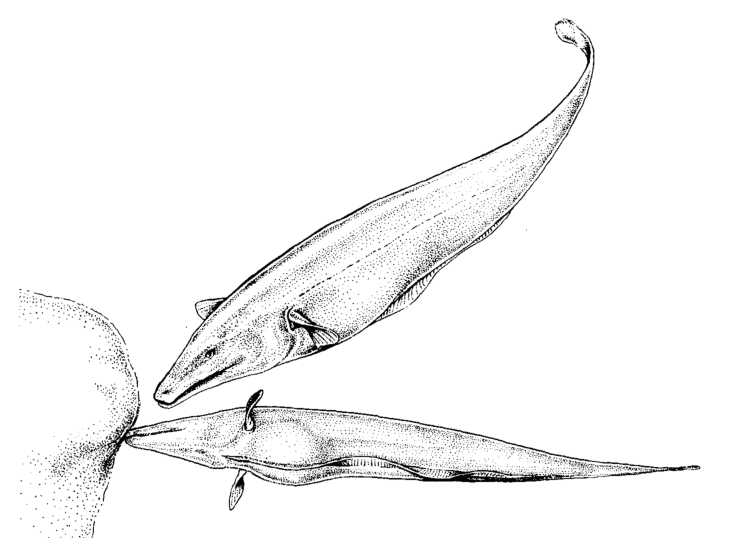
\includegraphics[width=.8\textwidth]{lepto_sketch}}
	\caption{\label{lepto_sketch} Physical appearance and mating behavior of \lepto{}. The characteristic enlarged ribbon fin enables these fish to swim in any direction independent from their orientation and helps them to maneuver in the confined spaces of their preferred natural habitats. Since the corresponding innervating muscles take up most of the caudal part of their  body, the visceral organs, including cloaca and gonads, are concentrated in the rostral body. The displayed behavior corresponds to reproduction. The coordination of females spawning a single egg and males fertilizing it is only one of the many social interactions, where electrocommunication is of central importance. Taken from \citet{Hagedorn1985}.}
\end{figure}

One of these interactions is competition behavior that, in \lepto{}, comprises ritualized fighting accompanied by various electrocommunication signals \citep{Triefenbach2008, Smith2013}. \lepto{} has been shown to mainly rival for optimal shelters whereas during mating season, males additionally compete for females \citep{Hagedorn1985, Dunlap2002, Henninger2018}. In both cases, more dominant individuals seem to have priority access. In staged competitions for single shelters, \citet{Dunlap2002} found more dominant individuals to occupy higher quality shelters, preferably alone, and anecdotal observations in the field and laboratory suggest more dominant males to participate more in reproduction (\citealp{Hagedorn1985, Henninger2018}, \figrefb{lepto_sketch}). 

Many previous studies found evidence for dominance hierarchies across populations of various electric fish species \citep{Dunlap2002, Stamper2010, Fugere2011, Silva2012}. Even though body size has been shown to be the main determinant for dominance and the outcome of associated competitions \citep{Dunlap2002, Triefenbach2008, Silva2012}, the influence of other factors including sex and the emission of various signals still remains unclear. Especially the role of an individual's EODf as indicator for dominance is discussed controversially. For \lepto{}, some studies found dominance to correlate with EODf in males, but not in females \citep{Hagedorn1985, Dunlap2002}; a finding that has been reproduced in a wild population of Sternarchorhynchus \citep{Fugere2011}. However, in males EODf also correlates with body size, and could therefore be a secondary characteristic of dominance \citep{Dunlap2002, Triefenbach2008, Fugere2011}. Furthermore, some studies suggest female electric fish to either form no dominance hierarchy at all \citep{Hagedorn1985} or only a very distinct one, whereby females with lower EODf are more likely to be found outside of shelter tubes \citep{Dunlap2002}. Other studies suggest dominance to be independent of sex \citep{Silva2012, Zubizarreta2020}. 

\subsection{Electrocommunication}

\begin{figure}[h!]
	\centerline{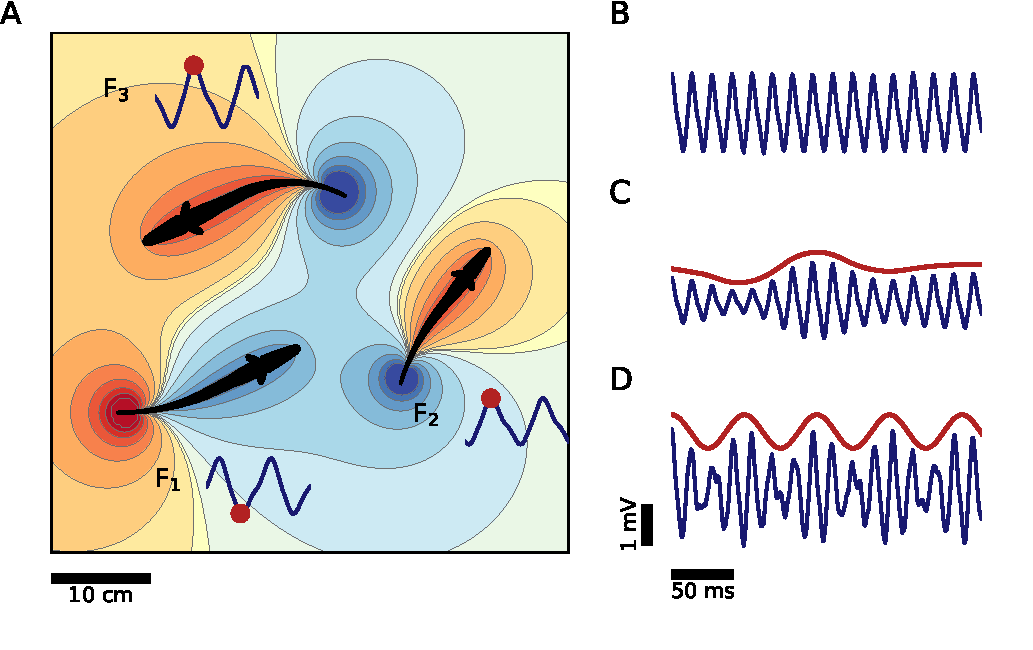
\includegraphics[width=.9\textwidth]{field_simulation}}
	\caption{\label{field_simulation} Electric field characteristics and interactions in electric fish \figitem{A} Electric fields of different fish superimpose and influence each others spatial properties. For each fish the current extend and direction of its electric field is dependent on the phase of its EODs (red marker in black EOD waveform). In the displayed state, the electric field of fish F$_1$ is anti-phasic to those of fish F$_2$ and F$_3$. However, this is only a short lasting state since each fish emits its EODs at an individual specific frequency (EODf). \figitem{B} EODfs of single individuals remain remarkably stable over minutes, hours, and days. \figitem{C} Amplitude modulations (AM) of a single electric field recorded via external recording electrodes or perceived by other electric fish resemble the movements of the respective fish. The amplitude of an electric field decays exponentially with distance to the receiver \citep{Benda2020}. \figitem{D} When two (in the purpose of simplification) stationary electric fields superimpose, the frequency of the resulting amplitude modulation, also called beat, corresponds to the difference frequency between the two original signals. Characteristics of the beat, i.e. its frequency and amplitude, are an important source of social information for electric fish since it resembles a conspecific's identity (individual specific EODf), its movement behavior (AM), and even its communication behavior (EODf changes).}
\end{figure}

Electrocommunication is used in various social contexts across electric fish species \citep{Westby1970, Hupe2008, Silva2012, Smith2013}. Especially \lepto{} is known for its rich repertoire of various electrocommunication signals \citep{Smith2013}, e.g. employed in courtship \citep{Hagedorn1985, Henninger2018} and agonistic contexts \citep{Hupe2008, Triefenbach2008}. Wave-type electric fish already gather relevant information about each other by means of perceived structural changes of their own electric field resulting from the interactions with electric fields of other fish (\subfigref{field_simulation}{A}). The electric fields of two wave-type fish superimpose and result in a beat, i.e. a periodic amplitude modulation of the receiver's electric field. 

The amplitude of the beat indicates the distance between fish, whereas the frequency of the beat equals the difference between the two EODfs (\citealp{Henninger2020}, \subfigrefb{field_simulation}{C, D}). Both amplitude and frequency of amplitude modulations are encoded by electroreceptor afferents of the active electrosensory system \citep{Benda2006, Hupe2008b, Walz2014}. In the \lepto{} species group \citep{DeSantana2013}, EODf is sexually dimorphic with females having lower frequencies (600--750 Hz) than males (750--1000 Hz, \citealp{Meyer1987}). Thus, beat frequencies convey information about species affiliation and sex of another fish, e.g. if it is a competitor for limited resources or a potential mating partner, but this information is ambiguous \citep{Henninger2018, Henninger2020}. Because of the beat, conspecifics can detect each other over a distance of up to two meters \citep{Knudsen1975, Henninger2018, Henninger2020} and potentially assess each other's sex and dominance, as well as monitor each other's movement behaviors \citep{Davies1978, Fernald2014}. At the same time, low-frequency beats have been suggested to jam electrolocation signals \citep{Bastian1987}, posing a potential limiting factor to group density.

\begin{figure}[tp]
  \begin{minipage}[t]{0.45\textwidth}\mbox{}\\[-2ex]
    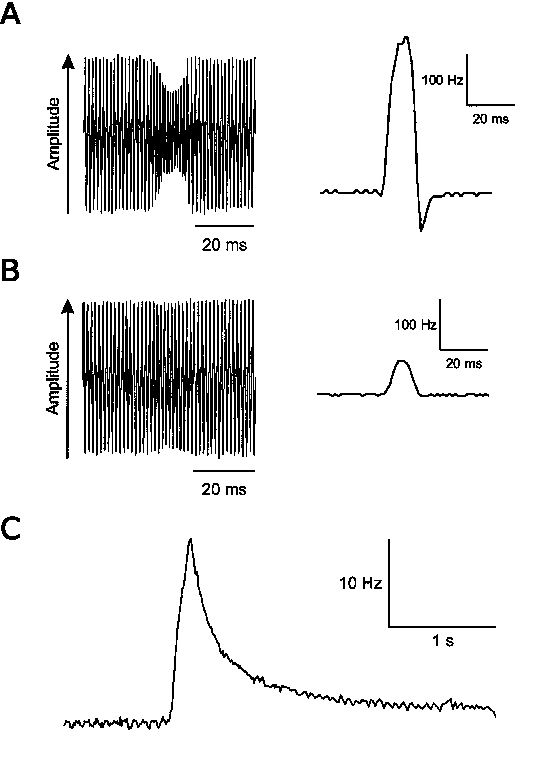
\includegraphics{e_communication}
  \end{minipage}
  \hfill
  \begin{minipage}[t]{0.35\textwidth}
  \caption{\label{e_com_sigs} Electrocommunication signals commonly emitted by \lepto{}. \figitem{A} Type-1 chirps are characterized by an EODf increase of up to 200\,Hz and a frequency undershot before returning to baseline EODf. While the chirp is emitted, the EOD amplitude is temporarily decreased. Type-2 chirps can best be elicited with EODs with large EODf difference, hinting towards their importance in inter-sex interactions. \figitem{B} Type-2 chirps are smaller in their frequency excursion and do not come with a decreased EOD amplitude. These chirps are emitted during agonistic interactions, but also during courtship. \figitem{C} Rises are characterized by rapid increases in EODf by a few tens of Hertz followed by an exponential decay back to baseline EODf. The significance of these signals is discussed controversially throughout the literature. Taken from \citet{Zupanc2002}.}
  \end{minipage}
\end{figure}

Wave-type Gymnotiform fish generate three distinct types of communication signals by actively modulating their EODf: Chirps, rises, and jamming avoidance responses \citep{Engler2000, Zakon2002}. Chirps are brief temporal frequency excursions ranging from 70\,Hz up to more than 400\,Hz with a duration of approximately 30\,ms to 500\,ms \citep{Engler2000} that transiently advance the phase of the ongoing beat \citep{Benda2005}. For \aptero{}, at least two types of chirps are known \citep{Hagedorn1985, Dunlap2003b, Henninger2018}. A small chirp (50--150\,Hz, \subfigrefb{e_com_sigs}{B}) is associated with agonistic, same sex interactions \citep{Smith2013}, but is also used during courtship to synchronize spawning \citep{Henninger2018}. A large chirp (200--400\,Hz, \subfigrefb{e_com_sigs}{A}) is predominantly produced by males in response to electric fields belonging to potential mating partners \citep{Triefenbach2003}. In \rostratus{} and \lepto{}, females exclusively produce a special long chirp when ejecting a single egg \citep{Hagedorn1985, Henninger2018}. However, it is important to note that most of the knowledge on chirps is based on laboratory experiments in more or less artificial and restricted settings (e.g. \citealp{Engler2001, Dunlap2003b, Zupanc2006, Hupe2008}). Those settings turned out to evoke chirping behaviors quite distinct from field observations or long term laboratory breeding experiments \citep{Henninger2018}. 

Another category of electrocommunication signals, EODf rises, are characterized by a rapid but moderate increase in EODf by no more than a few tens of Hertz followed by an exponential decay back to baseline EODf within a few seconds (\citealp{Hagedorn1985, Engler2000, Zakon2002}, \subfigrefb{e_com_sigs}{C}). The frequency increase and duration of rises are highly variable within species, but seem to be conserved across species and sexes \citep{Turner2007}. The function of EODf rises is discussed controversially \citep{Smith2013}. Rises have been suggested to be signals of dominance \citep{Tallarovic2005}, appeasement signals produced by subordinate fish \citep{Serrano2003}, context specific signals produced by subordinates and dominants \citep{Hopkins1974}, or just a general expression of stress \citep{Smith2013}.

Finally, in \Eigenmannia{}, electrolocation performance is impaired by the presence of a conspecific with a similar EODf \citep{Heiligenberg1973} because the resulting low-frequency beat shadows signals evoked by objects \citep{Behrend1977}. By means of the jamming avoidance response, \Eigenmannia{} changes its EODf in a way that the beat frequency is increased \citep{Watanabe1963, Bullock1969} and, thus, a jamming signal is moved outside the frequency band relevant for electrolocation \citep{Nelson1999, Fotowat2013}. In contrast, \aptero{} only increases EODf when jammed \citep{Heiligenberg1996}, which does not necessarily result in an increase of beat frequency, but instead sometimes actively jams a conspecific \citep{Tallarovic2005, Triefenbach2008}. The latter behavior might be considered a communication signal. However, its importance still remains to be determined.

\section{Aim of the study}

\lepto{} has been a successfully established model species in neuroscience for several decades. Even though their electro-sensory system is among the best described neuronal pathways (e.g \citealp{Benda2005, Bullock2006, Sinz2020}), little is known about their natural behaviors, including their social organization. Only few previous studies investigated behavioral topics like shelter occupation \citep{Dunlap2002, Stamper2010}, short competitions \citep{Hupe2008, Triefenbach2008}, dominance \citep{Dunlap2002}, and electrocommunication \citep{Smith2013, Henninger2018}, especially with chirps \citep{Engler2000}. Furthermore, most of these studies have been conducted in confined laboratory settings with reduced, artificial environments and short observation times. Accordingly, the interpretations of observed behaviors and suggested causalities are often conflicting between studies, but nevertheless provide a strong basis. Indeed, some studies started to evaluate behaviors of \lepto{} in the wild, focusing especially on movement patterns and intra-specific communication with chirps in the context of reproduction and aggression \citep{Henninger2018, Henninger2020}. However, in these studies the dimensionality of firm conclusions about the social organization in \lepto{} is limited since they lack information about the observed animal's physical conditions, life history, and long term behavioral traits (fish frequently leave observation areas and are impossible to reidentify). Many mysteries about their secretive life still remain unresolved: What form of social organization prevails in populations of \lepto{}? What external and internal motivators drive decision making during competitions for resources and dominance? What are behavioral manifestations of dominance? What is the meaning of the various electrocommunication signals involved in all kinds of social interactions?    

To explore these questions my thesis pursued two main objectives. First, I developed the methods and algorithms required for tracking EODs of individual wave-type electric fish recorded with electrode arrays in different laboratory and natural settings (\chapref{Methods}). I combined and refined previous approaches \citep{Madhav2018, Henninger2020} and thereby developed a semi-automatic system capable of tracking electric fish with unprecedented accuracy. This advanced tracking approach, accordingly, also reduces the expense of required post-processing and therefore facilitates long-term observation studies on electric fish in more naturalistic settings, i.e. when many with potentially similar EODfs are recorded simultaneously.

Subsequently, I applied the developed methods to observe and evaluate behaviors of freely moving and interacting \lepto{} in different settings. In order to gain a comprehensive understanding about the meaning and causalities of the various social behaviors of \lepto{}, I combined behavioral observations in naturalistic settings with controlled laboratory experiments. In a large laboratory aquarium containing several naturalistic habitats and shelters, I evaluated individual spatio-temporal behaviors in a population of 14 \lepto{} in order to tackle questions regarding habitat preference and group dispersion, as well as how a fish's spatio-temporal behavior is affected by its social status (\chapref{Habitats}, \citealp{Raab2019}). In a subsequent experiment, I analyzed behaviors and interactions of unfamiliar pairs of \lepto{} during staged competitions, e.g. when fish first try to establish dominance (\chapref{Competitions}, \citealp{Raab2021}). In this experiment, my main objective was to identify which individual characteristics or physical attributes of fish are decisive for the outcome of competitions, how fish assess opponents, and how this assessment manifests behaviorally. Another aim of this study was to identify the meaning of electrocommunication with rises during social encounters, especially in the context of agonistic interactions. 


%\bibliographystyle{jneurosci}
%\bibliography{../journalsabbrv,../references}